\pagenumbering{arabic}
\setcounter{page}{1}
\section{Introduction}
\subsection{Overview}
\subsubsection{Artificial Intelligence}
Artificial Intelligence (AI) is widely used in today's industry. It is an emerging field where machines are empowered to mimic human thinking, decisions and actions, to increase industries productivity in the sense of higher-level cognitive processing. In the not so distant past where robotics were programmed and used in manufacturing, today robotics incorporate not just programmed logic but also trained experience via continual exposure to external stimuli, action feedback and judgement adaptation to make a decision even on abstract information. For example, in the field of image classification, images are a 2D array of data. In a traditional programmable logic computing, it is architecturally impossible to recognize its unstructured content as it only deals with well defined, structured data. However, with new AI architecture like a neural network, it is possible to leverage the similar and minimalistic structural architecture of a human brain, to efficiently and precisely deal with the processing of such data. The more complex structure would mean a better ability to extract subtler and finer details. Based on these details, the classification of images can then be made. In the medical field, we have a classification of images for the presence or severity of the tumour. In the search engine, we have a classification of images for objects, scenery, etc. In a self-driving vehicle, we also have a classification of images for objects on road (See Figure \ref{fig:cvroad}).
\begin{figure}[H]
	\centering
	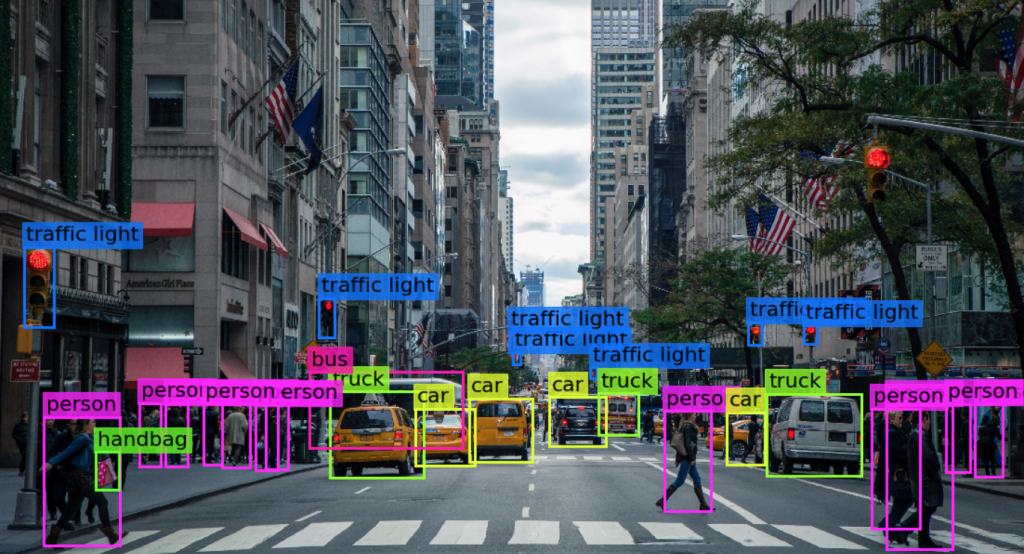
\includegraphics[scale=0.4]{cvroad.png}
	\caption{Objects recognised by AI on the road \cite{cvroad}}
	\label{fig:cvroad}
\end{figure}

Beside image classifications, AI is widely used in control and actuation. In a self-driving vehicle, AI can process data collected from its surrounding through different types of sensors, not just data from the objects to recognise their presence, but also data from intrinsic measurable, like distance to those objects and their trajectories, to steer the vehicle in the right direction and away from danger. For example, if a child suddenly ran out from nowhere on the road, an AI can force the vehicle to stop, and effectively avoid an accident.
\subsubsection{Biological Neural Network}
\begin{figure}[H]
	\centering
	\subfloat[A biological neural network]{
		\centering
		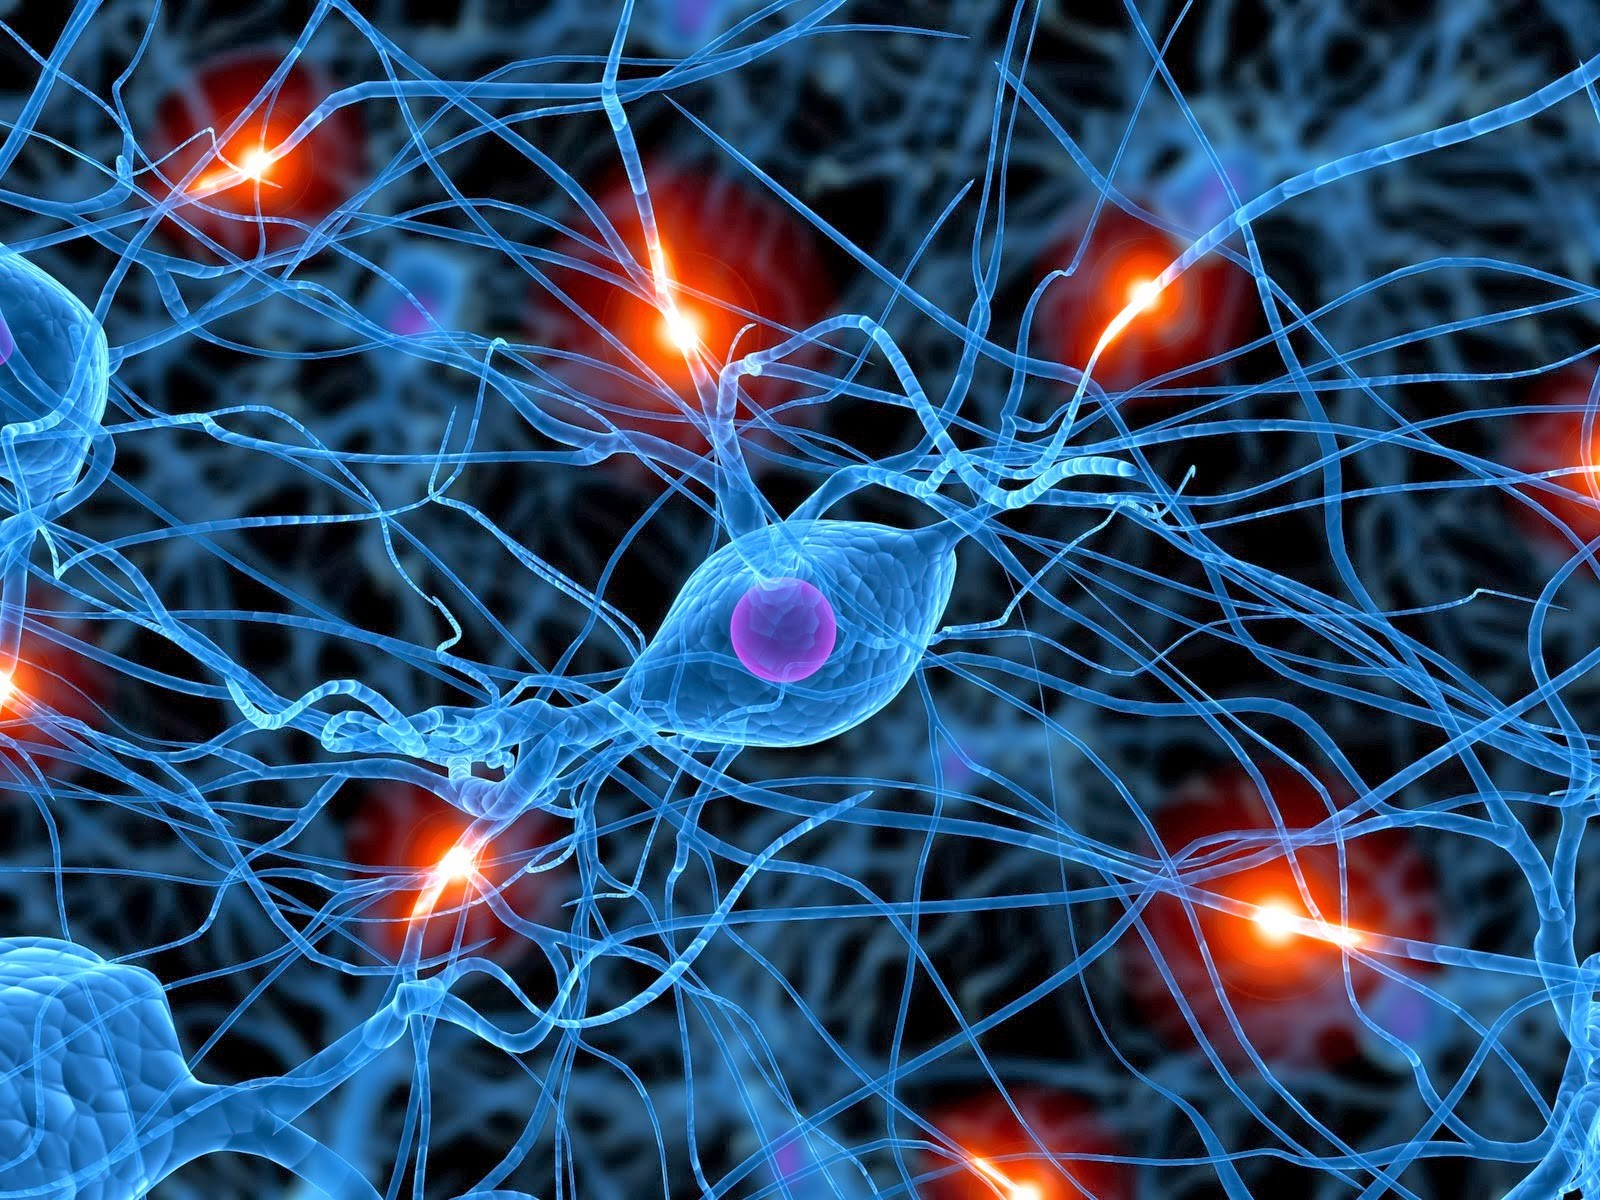
\includegraphics[scale=0.2]{bionetwork.jpg}
		
	}
	\subfloat[A biological neuron]{
		\centering
		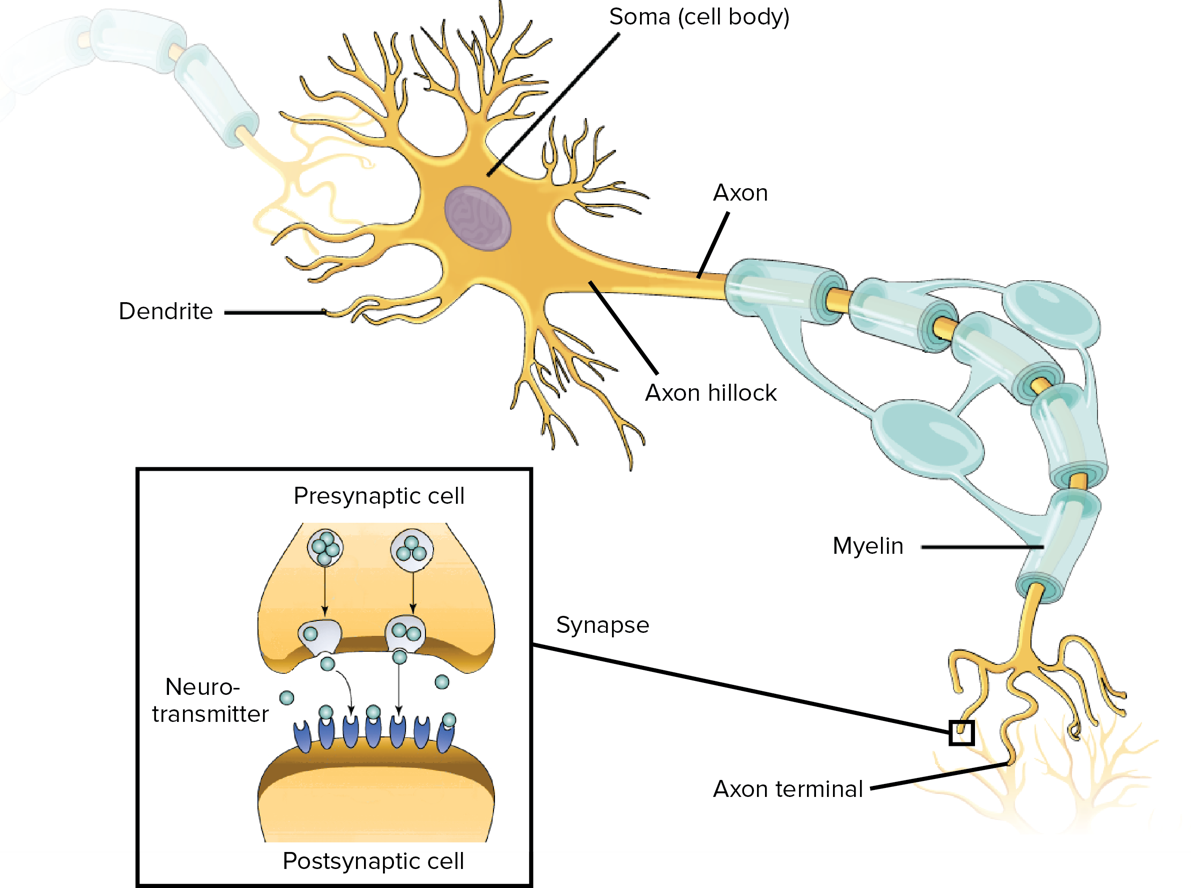
\includegraphics[scale=0.4]{biofullneuron.png}
	}
	\caption{Operational amplifier (opamp) characteristics}
	\label{fig:bionetwork}
\end{figure}
The biological neural network (Figure \ref{fig:bionetwork}) found in a human brain structure is extremely complex. A human brain contains more than 8 billion neurons and more than 100 trillion synapses (the connection between neurons). A neuron is a nerve cell that communicates with other cells via nerve impulses. It receives signals from one end known as dendrites, processes them via a mechanism known as an action potential, and send signal via elongated axon to another end. For the signal to pass from this terminal to the next neuron dendrite, it has to cross between a gap known as the synapse. The synapse can grow weaker or stronger over time, determining the strength of the synaptic connection, known as neural plasticity.

A neuron maintains a negative voltage (i.e. polarized) across its membrane at $-70mV$. It is achieved by complex protein structures sitting on the membrane known as an ion channel and ion pump. Whenever there are stimuli from the dendrites, they are integrated over time. As these stimuli are not perfect spikes, their strength dies down through time. There are 2 types of stimuli, one is excitatory post-synaptic potential, while the other is inhibitory post-synaptic potential. We can thus think of them as plus signal and minus signal. When these signals of equal strength come together at the same time, they cancel out each other and the net effect on a neuron is 0. If the sum of stimuli has a net positive effect, they come into the action potential mechanism picture.

\begin{figure}[H]
	\centering
	\subfloat[Biological neuron membrane]{
		\centering
		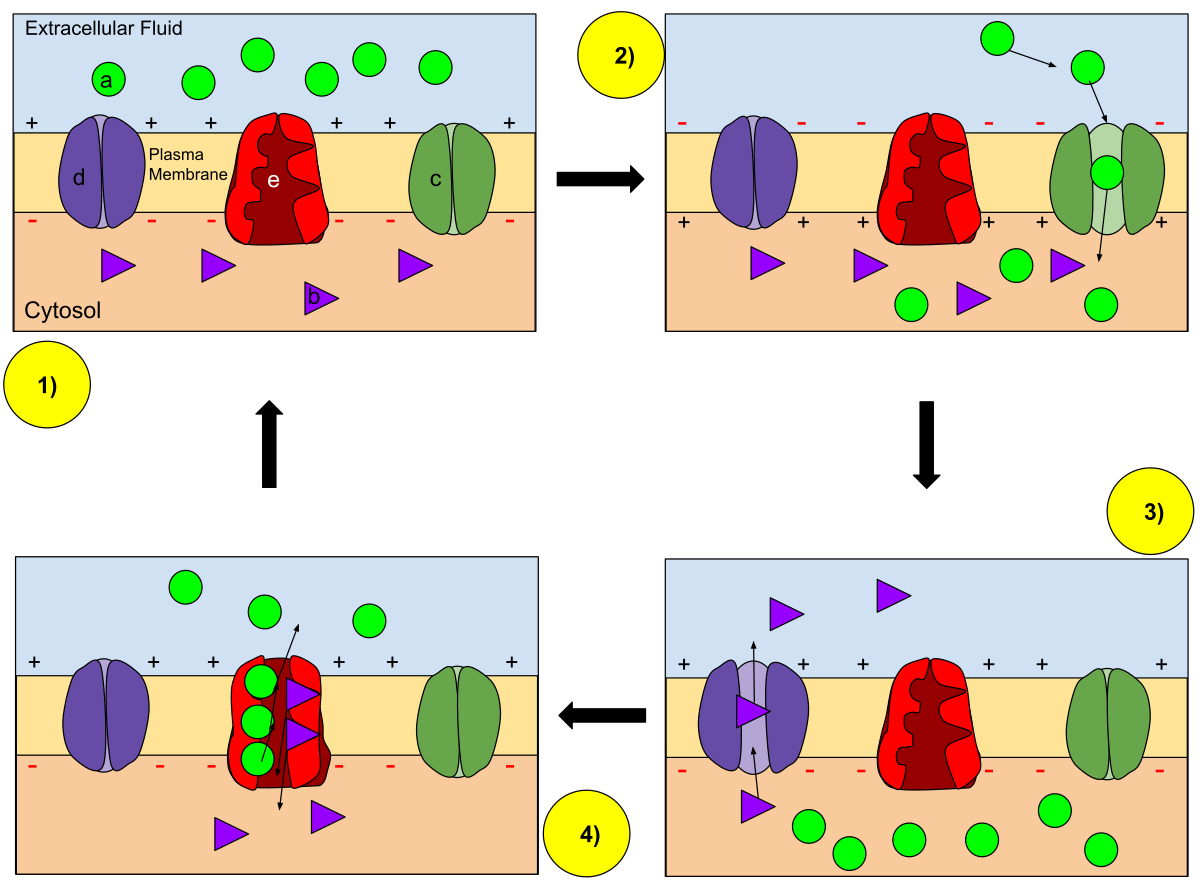
\includegraphics[scale=0.2]{bioneuron.png}
		
	}
	\subfloat[Action Potential]{
		\centering
		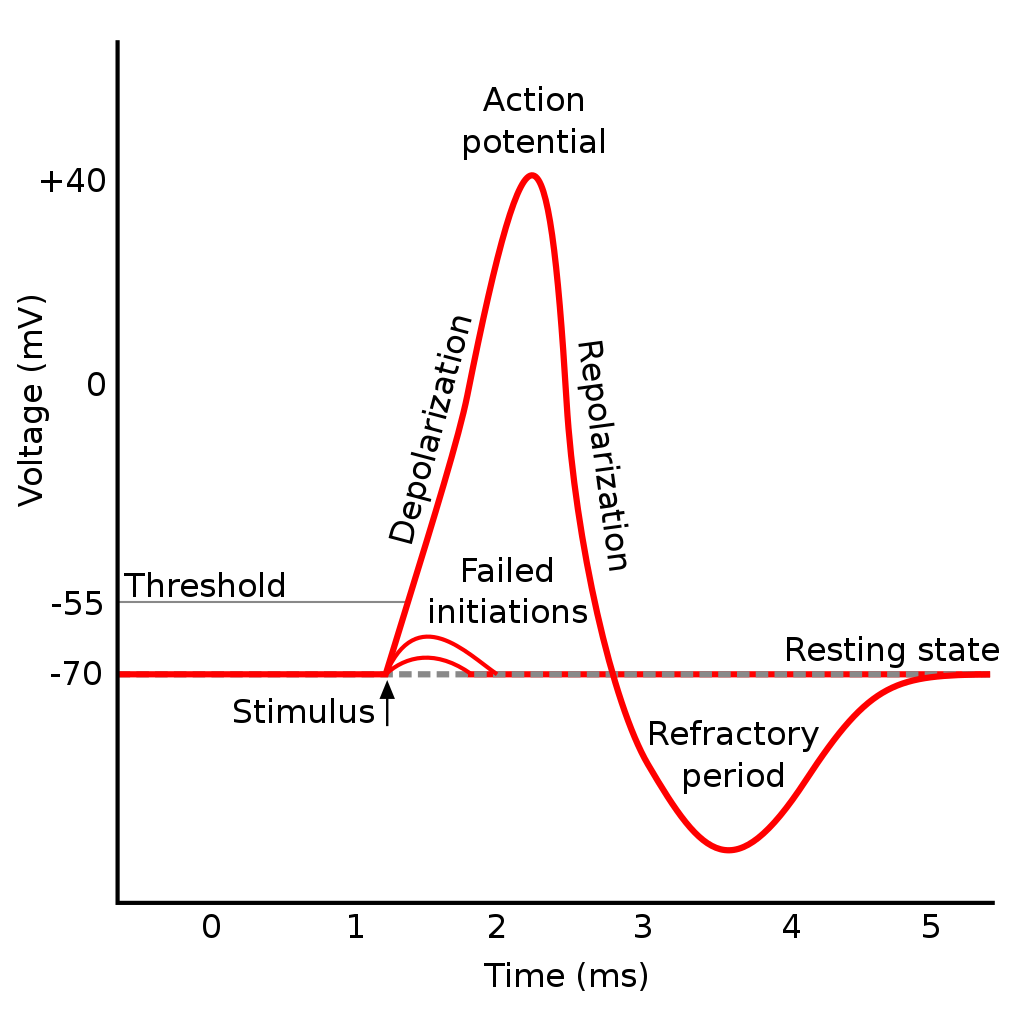
\includegraphics[scale=0.2]{actionpotential.png}
	}
	\caption{Across a neuron membrane}
	\label{fig:bioneuron}
\end{figure}

In Figure \ref{fig:bioneuron}, for a neuron to fire, i.e. generate a spike to other neurons downstream, the stimuli strength needs to cross the threshold at $-55mV$. Weak stimuli result in failed initiation action potential, whereas a strong stimulus results in depolarisation, triggering its action potential, peaking at about $+40mV$ before dropping back down, known repolarization. This repolarization process can cause its voltage to overshoot its initial negative voltage, before recovering to its resting state, known as the refractory period, and be ready for the next cycle.

In various stages of the action potential, the permeability of the neuron changes, as there are an exchange of ions. These are the 4 stages of an action potential cycle:
\begin{enumerate}
	\item Resting-State:\\
	Sodium ($Na^{2+}$) and potassium ($K^+$) ions have difficulty to pass through the membrane, and the neuron has a net negative charge internally.
	\item Depolarisation:\\
	This happens when the action potential is triggered. The sodium channels are activated, allow sodium ions to flow into the cell through the channel, resulting in a positive potential difference with respect to the extracellular fluid outside.
	\item Repolarization:\\
	This happens when the action potential peak is reached. The sodium channels close and potassium channel open, allowing potassium ions to flow out of the membrane through its channel into the extracellular fluid, reducing the membrane potential to a negative value.
	\item Refractory Period:\\
	The voltage-dependent ion channels are inactivated as the ions return to their resting distribution state across the membrane. The neuron is ready for the next action potential cycle.
\end{enumerate}
Memory is stored in the synaptic connection strength \cite{learnnmemory}, subjected to its plasticity. This plasticity exists for both short term and long term. Short term means this type of change only lasts for a time below a second before reverting to normal, whereas long term plasticity can last for years. Long term synaptic plasticity involves long term potentiation (LTP), i.e. strengthening or long term depression (LTD) i.e weakening. Intuitively, the frequent activity of synapse results in LTP, i.e. better memory, whereas prolonged infrequent activity result in LTD, i.e. memory loss. Neuron firing timing contributes to LTP and LTD too. For two neurons that are connected through a synaptic junction, if a pre-synaptic (i.e. previous) neuron fires $20ms$ or less before the post-synaptic (i.e. next) neuron, it results in LTP for the synapse connecting them. However, if a post-synaptic neuron fires $20ms$ or less before pre-synaptic neuron, it results in LTD. Hebbian theory, in particular, states that coincidental activity of synaptically connected neuron leads to lasting change in the effectiveness of synaptic transmission \cite{hebb}. In other words, it means neurons that fire together, are connected together.
\subsubsection{Artificial Neural Network}
\label{sect:ann}
An artificial neural network (ANN) is an architecture that mimics the human brain structure, which consists of synapses and neurons. Similarly, an ANN can receive inputs and process those input before reaching its outputs. Output can then be used for classification. For example, in a self-driving car, the input would be from the camera and sensors, and the output would be steering direction and magnitude and  acceleration. Input can be in many form, i.e. 1D vector or 2D matrix. Processing would then involve passing these input through many neuron layers, with each deeper hidden layer extracts subtler details (See Figure \ref{fig:nncomplex}).
\begin{figure}[H]
	\centering
	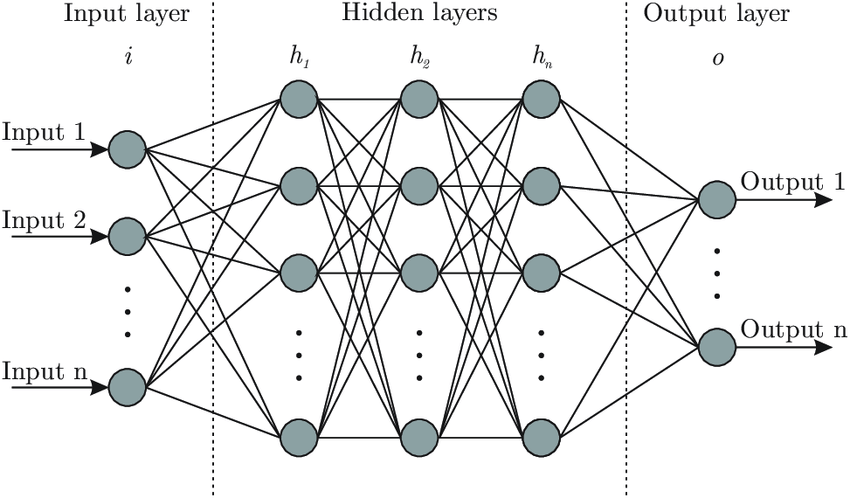
\includegraphics[scale=0.4]{nncomplex.png}
	\caption{Fully connected neural network overview \cite{rgnn}}
	\label{fig:nncomplex}
\end{figure}
For example, the input layer ($1^{st}$ layer) will have nodes/neurons with its numbers correspond to the number of inputs, i.e. 1D vector with $n$ elements would have $n$ number of inputs, whereas 2D matrix with $m\times n$ elements would have $m\times n$ number of inputs. In a fully connected layer (i.e. a dense layer), each neuron in the previous layer is connected to every neuron in the next layer. The connection between neuron A and neuron B is known as a synapse. Each of this synapse carries a weight and a stronger synaptic connection would mean a greater weight. This weight would then act on the input signal from the neuron to extract certain details. Basic processing is done as followed:
\begin{quote}
	\begin{figure}[H]
		\centering
		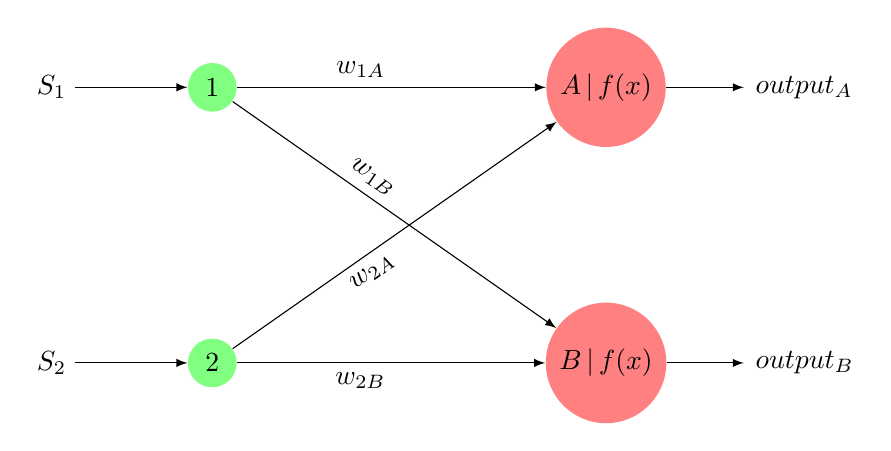
\begin{tikzpicture}[>=latex]
		\path
		+(0,0)  node[circle,fill=green!50]  (1) {$1$}
		+(0,-3.5)    node[circle,fill=green!50]  (2) {$2$}
		+(5,0)  node[circle,fill=red!50]  (A) {$A\,|\,f(x)$}
		+(5,-3.5)    node[circle,fill=red!50]  (B) {$B\,|\,f(x)$}
		;
		\draw[->] (-1.75,0)--(1) node[pos=0.1,label=left:$S_1$]{};
		\draw[->] (-1.75,-3.5)--(2) node[pos=0.1,label=left:$S_2$]{};
		\draw[->] (1)--(A) node[pos=.4,above]{$w_{1A}$};
		\draw[->] (1)--(B) node[pos=.4,sloped,above]{$w_{1B}$};
		\draw[->] (2)--(A)node[pos=.4,sloped,below]{$w_{2A}$};
		\draw[->] (2)--(B)node[pos=.4,below]{$w_{2B}$};
		\draw[->] (A)--(6.75,0) node[pos=0.9,label=right:$output_A$]{};
		\draw[->] (B)--(6.75,-3.5) node[pos=0.9,label=right:$output_B$]{};
		\end{tikzpicture}
		\caption{A simple artificial neural network illustration}
		\label{fig:nnillust}
	\end{figure}
	
	A layer is defined as a column of arrows, with/without weight attached, and usually ended with a column of neurons. Suppose in the input layer we have neuron 1 and neuron 2, and layer 2 we have neuron A and neuron B. Neuron 1 and neuron 2 synaptic connection to neuron A would be $w_{1A}$ and $w_{2A}$ respectively. Likewise, neuron 1 and neuron 2 synaptic connection to neuron B would be $w_{1B}$ and $w_{2B}$ respectively. Let say after layer 2 is the output layer:
	\begin{enumerate}
		\item Neuron 1 and neuron 2 receive signal $S_1$ and signal $S_2$
		\item Before reaching neuron A, by multiplying with the synaptic weight, the 2 signals become $net_A=S_1\times w_{1A} + S_2\times w_{2A}$
		\item Before reaching neuron B, by multiplying with the synaptic weight, the 2 signals become $net_B=S_1\times w_{1B} + S_2\times w_{2B}$
		\item The 2 signals for neuron A can be fed into an activation function $f(x)$, hence the output for neuron A becomes $output_A=f(net_A)$
		\item The 2 signals for neuron B can be fed into an activation function $f(x)$, hence the output for neuron B becomes $output_B=f(net_B)$
	\end{enumerate}
\end{quote}
Here, we are assuming that we already have the weight. i.e. the network is in inference mode. If we have defined inputs and desired corresponding outputs but without the weights, such that we need to figure out each weight, we can put the network into training mode to set the weight. A common way to work out the weights would be back propagation technique. In a simple back propagation technique, we would randomly set the weight of each of the synapses. Then, we inject signals into the input layer and measure the output from the last layer. We then compare the difference between the desired output and the output from the network, known as the error. From there, we can use partial differentiation to work out the error dependencies and tune the corresponding weight accordingly. The exact detail for back propagation technique for previous example is as followed:
\begin{quote}
	\begin{enumerate}
		\item Calculate error: $$E_{total}=E_{output\,A}+E_{output\,B}=\frac{1}{2}(desired_A-output_A)^2+\frac{1}{2}(desired_B-output_B)^2$$. Here, the purpose for the error for each of the output to appear in a halved and squared form is to simplify differentiation.
		\item we want to know how much $w_{1A}$ contributes to the total error $E_{total}$. Applying chain rule, we get:$$\frac{\partial E_{total}}{\partial w_{1A}}=\frac{\partial E_{total}}{\partial output_A}\times \frac{\partial output_A}{\partial net_A}\times \frac{\partial net_A}{\partial w_{1A}}$$
		\item As mentioned before in the $1st$ step, we use squared form to facilitate differentiation, here we have: $$\frac{\partial E_{total}}{\partial output_A}=-(desired_A-output_A)$$
		\item And, $\frac{\partial output_A}{\partial net_A}$ would depend on the activation function used, we will obtain a numerical value here too.
		\item Also, $$\frac{\partial net_A}{\partial w_{1A}}=S_1$$
		\item After obtaining numerical value for $\frac{\partial E_{total}}{\partial output_A}, \frac{\partial output_A}{\partial net_A}, \frac{\partial net_A}{\partial w_{1A}}$, we can finally have the value for $\frac{\partial E_{total}}{\partial w_{1A}}$.
		\item We can then proceed to set $$w_{1A\,(new)}=w_{1A\,(old)}-\eta\times \frac{\partial E_{total}}{\partial w_{1A}}$$ where $\eta$ is the learning rate. The smaller the value of $\eta$ ($<1$), the slower or more gradual the update is to the new value of $w_{1A}$, to prevent over adjustment. Over adjustment will lead to divergent behaviours, which is unfavourable especially if we aim to hit the minimum error spot. (See Figure \ref{fig:lrate}).
		\item we can repeat the same process above to set for $w_{1B},w_{2A},w_{2B}$.
	\end{enumerate}
	The same technique can be extended to $n$ layers fully connected network.
	\begin{figure}[H]
		\centering
		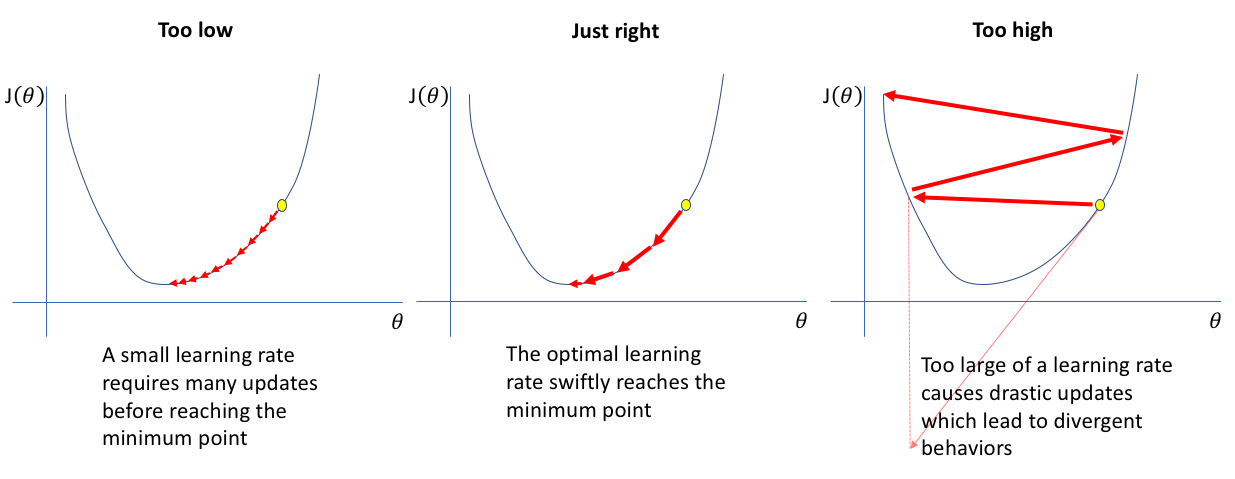
\includegraphics[scale=0.35]{lrate.png}
		\caption{Different learning rate and their contribution to the Cost Function $J(\theta)$ where $\theta$ is any parameter we want to optimize (e.g. weight $w$) and $J(\theta)$ is the function that computes Error $E_{total}$ \cite{lrate}}
		\label{fig:lrate}
	\end{figure}
\end{quote}
\subsubsection{von Neumann Computing}
In traditional computing, von Neumann architecture is being used. That means processing is only done in the central processing unit (CPU) and there constant shuttling of data between different memory device. There are mainly 2 types of memory devices on a traditional computing system, i.e. CPU cache and random access memory (RAM). A CPU cache is made up of expensive, superfast but small memory capacity whereas RAM is made up of slow but huge memory capacity. All neural network data are loaded to RAM before they are moved to the CPU cache for it to work with and the final processing result is stored back to the RAM. This long-distance bi-directional information flow between CPU and RAM constitutes most of CPU instruction cycles, consuming a huge amount of time and power (Figure \ref{fig:vonneumann}).
\begin{figure}[H]
	\centering
	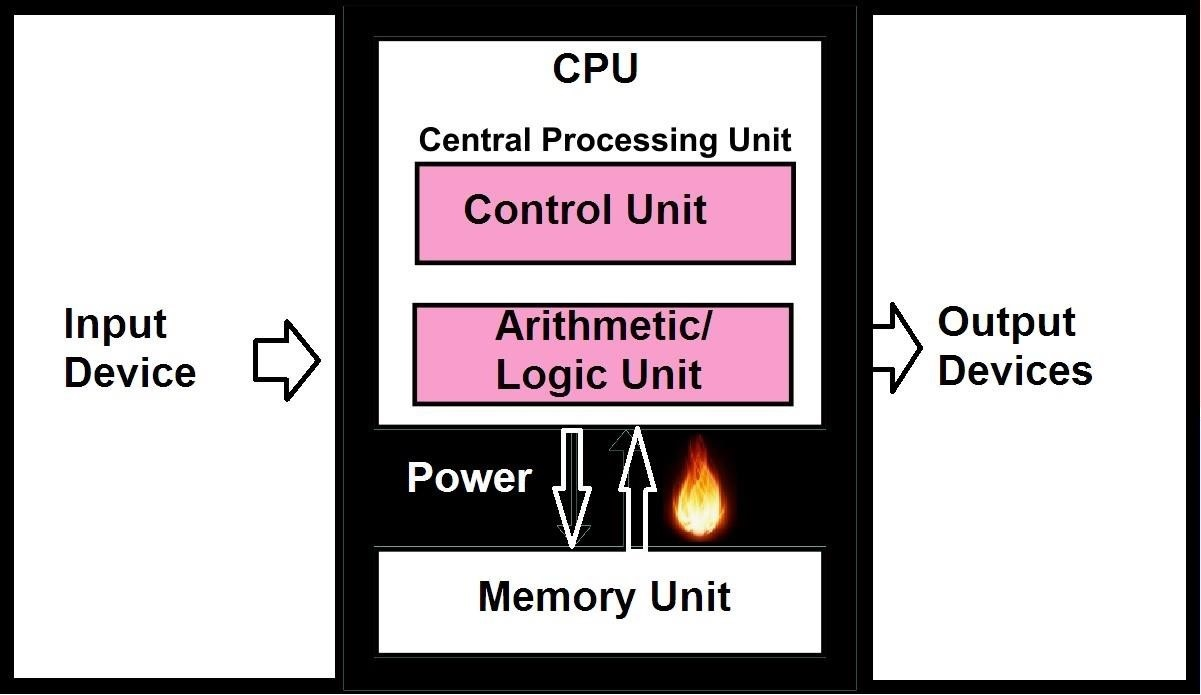
\includegraphics[scale=0.4]{vonneumann.jpg}
	\caption{von Neumann architecture}
	\label{fig:vonneumann}
\end{figure}

Neuromorphic computing comes into rescue when we have processor specially designed for neural computing. Although information can be analogue/digital, the processing is done with analogue processing. For example, a typical neural network involves summing and multiplication. On a von Neumann architecture, the process flow goes like this:
\begin{quote}
	Let say we are summing number $a,b,c$:
	\begin{enumerate}
		\item Load number $a$ from RAM to CPU register 1
		\item Load number $b$ from RAM to CPU register 2
		\item Sum $a$ and $b$ on CPU and store the result in register 3
		\item Save the value of $a+b$ in CPU register 3 to RAM
		\item Load value of $a+b$ from RAM to CPU register 1
		\item Load number $c$ from RAM to CPU register 2
		\item Sum the value of $a+b$ and $c$ on CPU and store the result in register 3
		\item Save the value of $a+b+c$ in CPU register 3 to RAM
	\end{enumerate}
\end{quote}
We would require so many steps to compute a simple summation, nevermind that CPU has billions of cycles to take care of these steps.
\subsubsection{Neuromorphic Computing}
\begin{figure}[H]
	\centering
	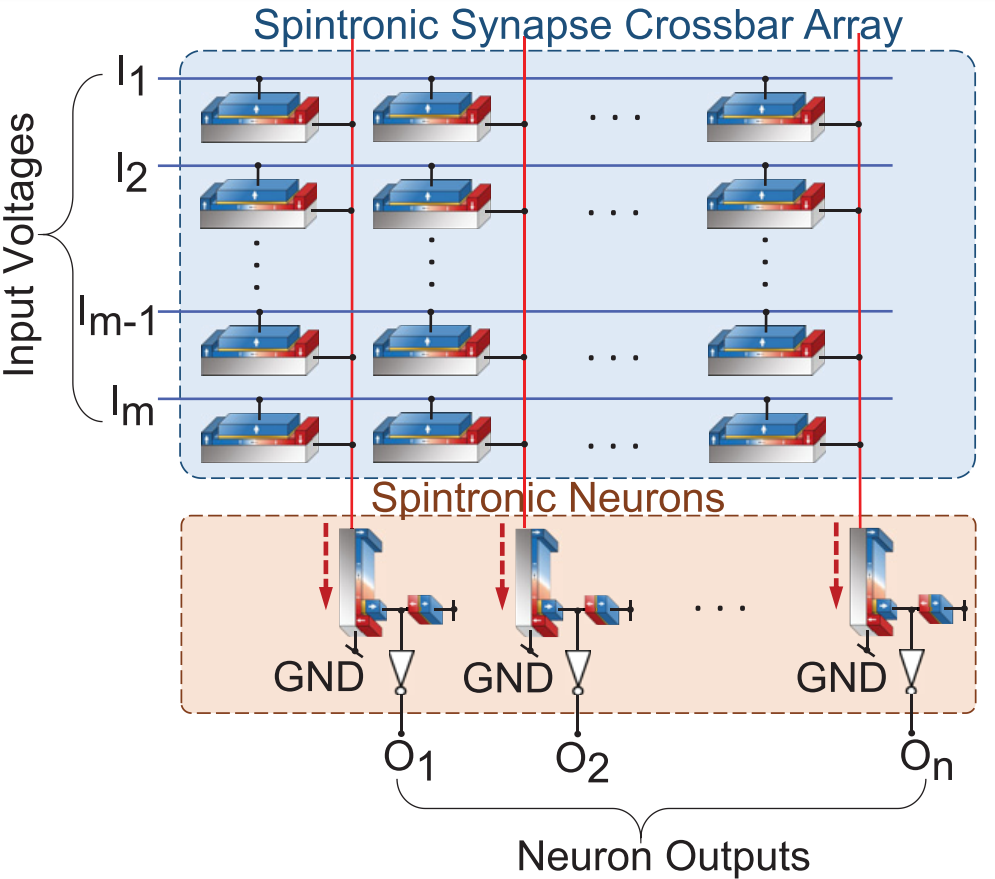
\includegraphics[scale=0.4]{neuromorphic.png}
	\caption{Neuromorphic architecture}
	\label{fig:neuromorphic}
\end{figure}
In neuromorphic computing (Figure \ref{fig:neuromorphic}), highly specialized circuits are used to do the computation and physical laws like fundamental circuit laws are leveraged. Simple mathematical computation like multiplication and summing that take many processing steps and cycles in von Neumann computing is now irrelevant because Ohm's law is used to do the multiplication and Kirchoff's current law is used to do the summation in massive parallelism, which is an operation known as in-memory computing.

However, due to the non-programmable, non-sequential processing and highly specialized nature of the circuit, it is designed solely for this purpose. It cannot run the software as von Neumann architecture does, so we can forget about running a computer operating system, watching YouTube videos, checking email, etc. Such circuit is known as an application-specific integrated circuit (ASIC). One such example is IBM TrueNorth chip, it consumes as little as $1/10000th$ the power of a traditional von Neumann computer.

What it lacks in its functionality, it more than makes up for in performance in terms of speed and power consumption. Multiple steps in a simple computation in von Neumann architecture that can scale easily up to millions of steps depending on the number of inputs can deter the network efficiency and its response in realtime because the time in sequential computation all add up to a prohibitively large delay. In contrast, all these sequential steps are reduced to a single step in neuromorphic computing architecture as the circuit laws naturally take care of these computations, less the need for purposeful sequential processing.

One notable development in neuromorphic computing is a spiking neural network (SNN). Unlike Von Neumann architecture, that is always on and all instruction executions are synchronized to the CPU clock cycle, SNN is event-driven, i.e. it performs computation and consumes power only when there are external stimuli, and there is no clock cycle to synchronized to. Furthermore, this SNN takes in signals in a form of spikes, unlike all other neuromorphic networks that take in signal in constant signal strength. That is how its power consumption is reduced significantly. Its computation method is biologically inspired, in a way that spikes from the external stimuli are received and accumulated in a neuron, and when a threshold is reached, the neuron will generate a spike to other neurons connected to it through a network of synapses.
\subsubsection{Spintronics for Neuromorphic Computing}
Spintronics make use of electron spin (orientation) to change its resistance. Spin Hall Effect (SHE) is used to write to the spintronic device, whereas Spin Torque Transfer (STT) is used to read the value from the device, in a form of a current (Figure \ref{fig:sttshe}).


\begin{figure}[H]
	\centering
	\subfloat[Separate write and read path \cite{spoteu}]{
		\centering
		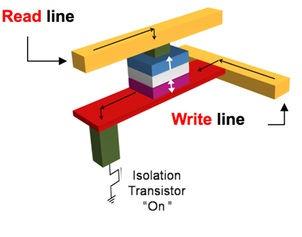
\includegraphics[scale=0.5]{sttshe.jpg}
	}
	\subfloat[Field free switching write operation]{
		\centering
		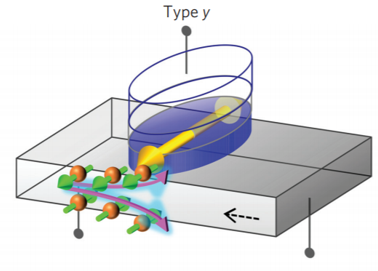
\includegraphics[scale=0.5]{shewrite.png}
	}
	\caption{SHE/SOT MRAM}
	\label{fig:sttshe}
\end{figure}

In a SHE write operation, when a current consisting of spin up and spin down electron, flowing through a heavy metal (HM) conductor in either direction, the electric field near the atom deflect spin up and spin down electron (much like sorting) to the edge of the conductor according to the spin. So, we can see spin up electron gather along one side or the conductor, whereas spin down on the opposite side. A different direction of current flow will see swapping side of previously mentioned electron spin (i.e. The side that consists of only spin up electron will now be replaced by only spin down, and vice versa). In the event with one side of the conductor is in contact with an electrode (Free layer), the electron spin in the HM can exert reorientation influence on the spin direction of the free layer.

Similarly, In an STT read operation, current consisting spin up and down electron flow through a normal conductor, but in a perpendicular/orthogonal direction from the top to the bottom. Since fixed layer has its electron spin pinned to one particular direction, when viewed together with electron spin in the free layer, we can observe them being parallel or antiparallel electron spin. Parallel spin results in lower resistance compared to that of antiparallel spin. After passing through and filtered by fixed layer (aligned spins pass through, whereas anti-aligned spin gets bounced), electrons have to tunnel through to a thin, insulating oxide layer to reach the free layer (electron antiparallel spin get bounced again here) to form a read current. This structure is known as a magnetic tunnel junction (MTJ) \cite{bhatti}.

\begin{figure}[H]
	\centering
	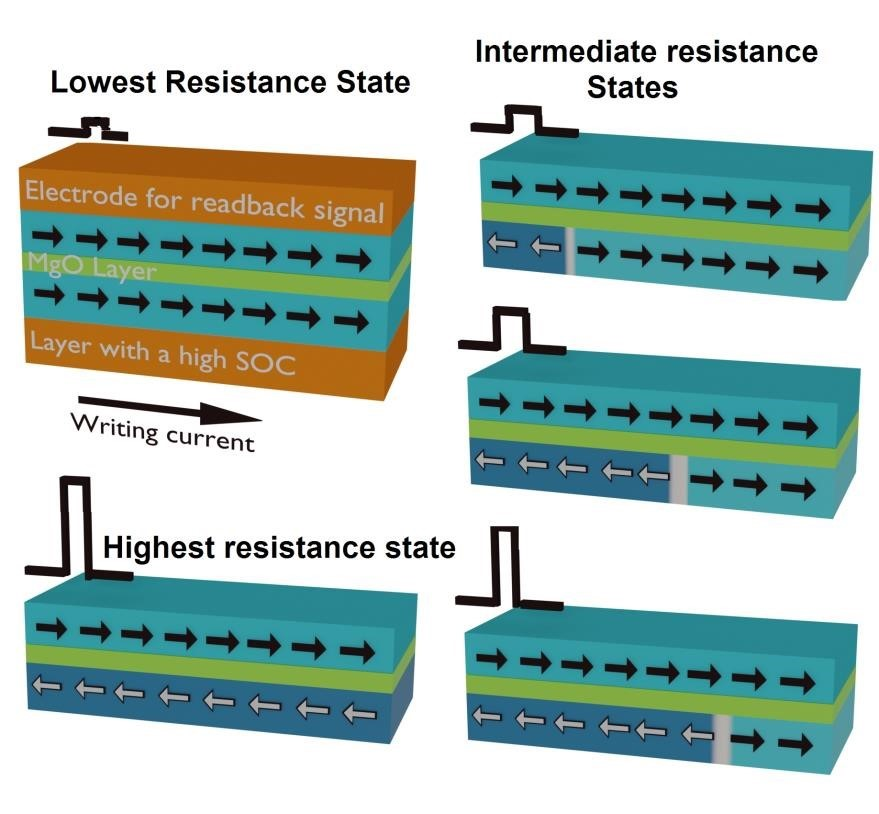
\includegraphics[scale=0.4]{dw.jpg}
	\caption{Domain wall device with multiple resistance states}
	\label{fig:dw}
\end{figure}

In a domain wall (DW) type MRAM (Figure \ref{fig:dw}), an MTJ has multiple resistance states instead of just 2 states (low and high). For this project, we consider 8 steps or equivalently 9 resistance states. These states comprise a fully antiparallel state, 7 intermediate states and a fully parallel state. To traverse between these states, multiple short SHE current pulses are applied, to move domain wall in step-like forward and backward fashion, until the desired resistance state is achieved. 

Simulation in this project only considers the resistance states of a DW MTJ, not a full simulation model (consisting of both writing and reading operation) because it is not available, and only recently under development by a PhD student.
\subsection{Background}
There have been numerous development in neuromorphic computing and spintronics.\\
For neuromorphic computing:\\
In 1957, there was an invention of the perceptron. Then there was the publication of very large scale implementation (VLSI) architecture for the implementation of the neural network after 29 years. In 1997, we saw the third generation of neural network - spiking neurons being published. There there was more neuromorphic silicon chip invented, mainly by IBM (TrueNorth chip in 2014) and Intel (Loihi chip in 2018).

For spintronics:\\
In 1989, the GMR effect is discovered in a thin film, GMR application of hard disk head by IBM in 1997. Around the same period, there was an advent of STT. Until recently, we have field-assisted MRAM and STT MRAM.
\subsubsection{Literature Review}
Different research papers were read and cross-referenced to have a better idea of this project. Concretely, they comprised of around 8 neuromorphic computing related papers, a spintronic paper, a neuromorphic spintronics review paper, and a domain wall based neuromorphic computing paper, with the latter most closely related to this project, supplied by both supervisor and co-supervisor.

A few papers touched on the material and device of crossbar array, involving physical metal oxide (MO) resistive ram (RRAM) by S. Yu et al \cite{yu}, a simulation model of MO RRAM by M.K.F. Lee et al \cite{lee}, physical Conductive-Bridge RAM (CBRAM) by M. Suri et al \cite{suri}, memristor by X. Liu et al \cite{liu}, domain wall MRAM by D. Kaushik et al \cite{kaushik} and spintronics by J. Grollier et al \cite{grollier}. They demonstrated the viability of such material and device used in a synapse. S. Yu et al. demonstrated the use of MO as synaptic device and the I-V relationship with multiple continuous SET cycles, followed by RESET cycles variation. These variations although is undesirable but are tolerated, much like what happens in a biological synapse. The performance requirement is more lenient than a digital data storage system because it is part of a massively parallel computing neuromorphic network. It is the collective effect of synapses that determine the firing of a single neuron, so individual variation has much less effect. Still, there is a need to limit these variations. However, shortcoming like 100000 endurance cycle limits the lifespan of the device. Nevertheless, this device consumes a meagre $6pJ$ per operation, and its property of gradual resistance change by pulse amplitude can be used for spike-timing-dependent plasticity phenomenon in an artificial neuron, similar to that of a biological one, and therefore can be used for the neuromorphic network \cite{yu}. M.K.F. Lee et al design an RRAM model, by making use of the non-ideality behaviour of the RRAM, they include Stuck-at-Faults where RRAM resistance value refused to change no matter what operation is done on it due to manufacturing defects, random telegraph noise where RRAM randomly fluctuate between 2 random states due to random trapping and release of charge carriers, as a result of lattice defects and write variability, where the RRAM resistance show random variability during SET/REST operation, due to migration of ionized defects that changes its physical dimension. Monte Carlo simulation was used to simulate the random telegraph noise. They attempted to mitigate write variability using a write-verify scheme and studied its trade-off \cite{lee}. M. Suri et al exploit CBRAM variability and stochasticity, which are originality undesirable characteristic to implement probabilistic learning rule. They demonstrated its use in auditory and visual applications with high accuracy, having audio sensitivity of $>2$, surpassing that of human and video detection rate $> 95\%$. The synaptic power consumed was ultra-low, with audio and video consuming $0.55\mu W$ and $74.2\mu W$ respectively. However, they found it hard to emulate long term depression behaviour using CBRAM due to difficulty in dissolving the conductive filament controllably. Hence, they decided to switch to binary (1-bit) to reduce the resistance representation resolution \cite{suri}. X. Liu et al indicated that memristor (a 2 terminal device which resistance varies as a function of electric charge and magnetic flux, made programmable by duration and amplitude of programming signal) of a same crossbar array row can be programmed all at once, and the positive implication reducing sneak path leakage \cite{liu}. D. Kaushik et al pointed out the advantage of using domain wall (DW) device programming compared to resistive random access memory (RRAM) phase-change memory (PCM) programming. In DW device, any resistive changes to the device are symmetrical whereas it is asymmetrical for RRAM and PCM device. Symmetrical means both positive and negative conductance changes of equal magnitude constitute the same pulse number and same energy required. It takes the same $0.18fJ$ for increase/decrease of conductance for DW, but $12pJ-51pJ/2.28nJ$ for increase/decrease of conductance for RRAM and $5pJ/30pJ$ for increase/decrease for that of PCM. Comparing the total power consumption for on-chip training, the power draws are $9fJ$, $1\mu J$ and $1.1\mu J$ for DW, RRAM and PCM respectively. For on-chip test performance, in ascending order of high accuracy, we have DW ($90\%$), PCM ($92\%$) and RRAM ($94\%$). They also noted the nucleation requirement at the beginning of the training for DW based neuromorphic network, hence the additional time and energy needed. Nevertheless, those energies are insignificant when compared to the total energy involved in training \cite{kaushik}. J. Grollier et al gave a review of spintronics role in neuromorphic computing. The main challenges are footprint and power consumption. Magnetic tunnel junction (MTJ) device is compatible with existing silicon chips manufacturing and can meet the need of small footprint and ultra-low power consumption. They investigate the role of MTJ as synapses and neurons and domain walls as neurons. They also note challenges of scaling up the system in a form of power consumption when more neurons are interconnected and the need for adapting the algorithms to the hardware when the reading of the small change of resistance is slow. They also indicated the possibility of employing low resolution 2 state MTJ device for inference mode with training mode in high-resolution \cite{grollier}.

A few involve employing an existing on-chip system to implement AI application, like a comprehensive study and benchmarking of various digital neuromorphic chips by H.F. Langroudi et al. \cite{langroudi}, full-custom hardware implementation by G. Indiveri et al. \cite{indiveri} and conversion of recurrent neural network (RNN) to SNN in IBM TrueNorth chip by P.U. Diehl et al \cite{diehl}. H.F. Langroudi et al. benchmarked 16 digital neuromorphic chip architectures and found out what optimization contributes to the improvement of performance. They realised the shrinking 16-bit to 8-bit or half the synaptic weight resolution only degrade the accuracy by $0.6\%$. This saves memory space and reduces computation complexity significantly, while only sustaining a slight reduction in accuracy. They further explored the possibility of binary (1-bit) resolution on a large dataset but discovered that it reduced by a significant amount. They noted the main optimizations are reducing memory power usage and its bandwidth grant high memory accesses. Input/Output communication overhead is often overlooked when reporting digital system performance (these overheads make up a portion of power usage and time delay) \cite{langroudi}. G. Indiveri et al implement analogue neuromorphic cxQuad (1k neurons and 64k synapses) and ROLLS chip (256 neurons and 128k synapses) with an asynchronous digital circuit. The energy consumptions for both neuromorphic chips at 30Hz operation are $945mW$ and $4mW$ at $1.8V$ respectively. Dynamic vision sensor (DVS) is first used for capturing visual input and it only responds to the changes in the scene. The cxQuad chip used digital circuits to route asynchronous spiking signal within the cores, and across the cores and chips. They pointed out that the analogue circuit is affected by device mismatch. The whole setup was aimed to solve von Neumann bottleneck issue \cite{indiveri}. P.U. Diehl et al stated the importance of RNN in temporal sequence learning and its difficulty in mapping and representing the network in spike-based architecture. They hence introduced a technique, known as train-and-constrain, to backpropagate the signal through time, before quantizing the weight and converting to SNN on a spike-based IBM TrueNorth chip. They conducted a case study on natural language processing (NLP) question classification and achieved $74\%$ accuracy, with only $0.025\%$ chip utilisation, and estimated power consumption of $17\mu W$ compared to traditional hardware like CPU and GPU which can consume at least $100W$ \cite{diehl}.

Those with purely neuromorphic network end-to-end simulation includes very efficient reconfigurable neuromorphic computing accelerator design by X. Liu et al \cite{liu}, domain wall-based synaptic neural network by D. Kaushik \cite{kaushik}, RRAM based neuromorphic computing by M.K.F. Lee et al \cite{lee} and conversion from an ordinary convolutional neural network (CNN) to spike-based neuromorphic (SNN) by Y.Q. Cao et al \cite{cao}. X. Liu et al demonstrated multilayer perceptron network, with 1st layer as the input layer, a middle layer as a hidden layer and an output layer as the last layer. Hidden layer involves summing at the neuron and applying a sigmoid activation function, known as a summing amplifier. They have router talking to memristor-based crossbar array, and they also imparted hybrid analogue and digital signal conversion in their network. They used the Cadence Virtuoso simulation environment. They made a comparison to a typical von Neumann based processor and their mixed-signal neuromorphic computing accelerator achieved $178.4\times (27.06\times)$ better performance and $184.2\times (25.23\times)$ better power efficiency, all while achieving similar computation accuracy \cite{liu}. D. Kaushik demonstrated the on-chip DW based neuromorphic network with all neuron output being feedbacked to the DW writing operation of synapses of the same column (only where the summing and multiplication operation are involved, as other columns are not involved in the operations at all). The feedback signal is comprised of a custom cost function after the pre-amplification and activation function. Here, the $R_F$ of the opamp is set to $1\Omega$ to ease the computation complexity. Due to long RESET duration pulse needed for RRAM/PCM, training of these network takes a longer time compared to that of DW type \cite{kaushik}. M.K.F. Lee et al attempted various spiked-based neuromorphic network setup by cascading the network, chaining the network in a ring fashion and pan out the network in a mesh-like fashion and discovered the highest performing type is cascade style network. They developed network architecture with multiple cores consisting of RRAM crossbar array with configurable network interface linking the cores and a router to route the information between them \cite{lee}. Y.Q. Cao et al employ steps like negative values elimination, ReLU for neuron activation and remove bias from all neural layers to convert ordinary CNN to tailored CNN, which can be easily converted to SNN. Their architecture involves preprocessing the image dataset into YUV colour space, generate spikes based on the colour values, passed through 2 units of convolution and subsampling layers, followed by a convolution layer and finally a fully connected linear classifier, all with spike-based neurons. The last layers utilised a spike counter to compare the count rate of the classifier outputs \cite{cao}.

A handful deal with SNN computing, involving its architectures by G. Indiveri et al \cite{indiveri}, conversion of recurrent neural network (RNN) to its spike-based form by P.U. Diehl et al \cite{diehl}, its application in object recognition by Y.Q. Cao et al \cite{cao} and spike-based neuromorphic simulation by M.K.F. Lee et al \cite{lee}. G. Indiveri et al implemented an adaptive-exponential-integrate-and-fire model to predict real neuron voltage traces and its dynamic behaviour. The synapse circuit of ROLLS chip employs synaptic behaviour like short term plasticity and long-term potentiation to account for the dynamics. They argued that embedded SNN system can deal better with realtime sensory processing application \cite{indiveri}. P.U. Diehl et al quantized the synaptic weight to 4-bit to accommodate the requirement of TrueNorth network parameter. To map to the spiking neurons, network rectified linear units (ReLU) are used without bias. When a spike is generated, the membrane voltage is reduced by a threshold voltage, a minimum voltage required for a spike event \cite{diehl}. Cao et al make use to converted SNN network to conduct case studies on Neovision2 Tower dataset and Cifar-10 dataset.  Neovision2 Tower dataset consists of objects like nontarget, bus, car, cyclist, person and truck for image recognition. The performance in accuracy for both datasets are $98.43\%$ and $99.29\%$ respectively \cite{cao}. M.K.F.Lee et al developed a simulation model for spiked based leaky-integrate-and-fire neuron to get a balance between accuracy and complexity and it is realisable in the hardware level \cite{lee}.

All papers assume the reader to have some level of foundation in training a neural network and testing its efficacy.
\subsection{Motivation}
Neuromorphic computing offers huge application in AI Computer Vision by mimicking human brain neuron and synapse network. It consumes very low power compared to von Neumann Computing and in-memory processing and hardware-based implementation of the neural circuit make it very efficient for visual object recognition. It can be designed to have multiple deeper layer network that extracts subtler visual details and its final network output can be fed for image classification.

Spintronic devices are originally used in hard disk drive read/write head. They are involved in:
\begin{enumerate}
	\item Spin Transfer Torque (STT)
	\item Spin Orbit Torque (SOT, Spin Hall Effect)
	\item Tunneling Magnetoresistance (TMR)
	\item Giant Magnetoresistance (GMR)
\end{enumerate}
for a magnetoresistive application like Magnetoresistive Random-access Memory (MRAM). They are non-volatile (information retention during power loss) like solid-state drive (SSD) unlike metal oxide semiconductor (MOS) and capacitors. Similar to SSD, magnetic tunnel junction (MTJ) uses electron tunnelling. The main motivation of using MTJ is it has a smaller footprint compared to that of CMOS. But, MTJ uses electron spin orientation instead of electron presence in SSD. Charge retention in a typical SSD changes its threshold voltage, causing wear out. In contrast, an MTJ offers a further advantage in higher read/write speed, lower power through flipping of electrons’ spin rather than the charge motion that tend to result in Joule heating and no wear out (Unlimited read/write cycle).

\subsection{Problem Statement}
A neuromorphic network is an efficient way to realise neural network, together with domain wall based MRAM with benefits like ultra-fast switching, ultra-low power consumption and excellent memory retention, therefore, it is very desirable to combine these two.
An ideal neuromorphic network involves an infinite range of resistance, vastly simplifying the design of the network, however, with the limited range resistance, an additional circuit is needed to overcome the shortcoming. In this study, we create and simulate models of neuromorphic network, taking into account the resistance range of domain wall based spintronic MRAM and compare the performance between neuromorphic model and traditional software implemented neural network model.
\subsection{List of Contribution}
In this final year project report:
\begin{enumerate}
	\item We show a basic construction of a neuron with circuit theory and derivations.
	\item We demonstrate Cadence Software implementation of an extended $n$ by $m$ scale neuromorphic circuit.
	\item We bridge the gap between theory and practical implementation.
	\item We showed a practical, foundry manufacturable, component level implementation of the neuromorphic circuit from actual third party foundry supplied 65nm process design kit, without resorting to the ideal model.
	\item We illustrate 4 versions of neuromorphic circuit.
	\item We compare and contrast the practical and ideal model with practical limitation.
	\item We explain sources of error in a practical model with detailed diagrams and equations.
	\item We demonstrate the training of different neural network models for a case study - MNIST handwritten digit database using open-source deep learning TensorFlow, Keras Library.
	\item We cherry-pick the best model most suited for transferring to neuromorphic network, with high accuracy.
	\item We use computer vision library - OpenCV to demonstrate the result of neuromorphic circuit output for our case study.
	
\end{enumerate}